% --- EJEMPLO CON LATO ---
\documentclass{article}
\usepackage[T1]{fontenc} % Codificación de fuentes mejorada
\usepackage{lato}        % Carga la fuente Lato
\renewcommand{\familydefault}{\sfdefault} % Hace que la fuente por defecto sea Sans-Serif

\usepackage[spanish]{babel}
\usepackage{amsmath,amsfonts,amssymb}
\usepackage{booktabs}
\usepackage{longtable}
\usepackage{array}
\usepackage{geometry}
\usepackage{fancyhdr}
\usepackage{hyperref}
\usepackage{setspace}
\usepackage{threeparttable}
\usepackage{dcolumn}
\usepackage{multirow}
\usepackage{pdflscape}
\usepackage{afterpage}
\usepackage{capt-of}
\usepackage{float}
\usepackage{subcaption}
% --- PAQUETES NECESARIOS PARA LA TABLA ---
\usepackage[utf8]{inputenc} % Para poder usar tildes, eñes y otros caracteres en español
\usepackage{tabularx}      % Para el entorno 'tabularx' y la columna 'X'
\usepackage{natbib}        % Para el comando de citas '\citet'
\usepackage{graphicx}      % Necesario para \textwidth en algunos casos
\usepackage{ragged2e}      % Para un mejor justificado en columnas 'X'

% --- Configuración opcional para las citas (si usas natbib) ---
\bibliographystyle{plainnat} % Estilo de bibliografía




\geometry{margin=2.5cm}
\onehalfspacing

\title{\textbf{Replicación y Extensión de Pavia et al. (2017): \\Evaluación de la Calidad de las Añadas de la Contabilidad Nacional Trimestral Española con Análisis del COVID-19}}

\author{
    Manuel A. Hidalgo-Pérez\thanks{Universidad Pablo de Olavide, Sevilla. Email: mhidper@upo.es} \\ 
    \textit{Universidad Pablo de Olavide} \\[0.5em]
    \and
    Leandro Navarro Pablo\thanks{Autoridad Independiente de Responsabilidad Fiscal (AIReF). Email: lnavarro@airef.es} \\
    \textit{AIReF}
}

\date{\today}

\begin{document}

\maketitle

\begin{abstract}
\noindent La fiabilidad de las estimaciones económicas preliminares es crucial para la toma de decisiones y la investigación. Este estudio realiza una doble contribución al análisis de la calidad de los datos de la Contabilidad Nacional Trimestral (CNTR) en España, tomando como referencia el trabajo seminal de Pavia et al. (2017). Primero, se lleva a cabo una replicación metodológica exhaustiva de su análisis para el período original 2005-2016, validando sus hallazgos clave, como la mayor precisión de las estimaciones del cuarto trimestre para las tasas de crecimiento interanual. Segundo, el análisis se extiende hasta 2025, lo que permite evaluar el comportamiento de los errores de revisión durante episodios de estrés económico sin precedentes. Nuestros resultados revelan una heterogeneidad notable en el impacto de las crisis; mientras que la pandemia de COVID-19 amplificó los errores de revisión en un factor de 2,94, este impacto fue superado por el de la crisis de deuda soberana (3,59). Al implementar todo el análisis en código Python de acceso abierto, no solo garantizamos la reproducibilidad total del estudio, sino que también ofrecemos una herramienta robusta para futuras investigaciones.

\noindent \textbf{Palabras clave:} Contabilidad Nacional, Revisiones de Datos, Replicación, COVID-19, Estadísticas Económicas

\noindent \textbf{Códigos JEL:} C82, E01, E32
\end{abstract}

\newpage

\section{Introducción}

La calidad y fiabilidad de las estadísticas económicas oficiales constituyen pilares fundamentales de la política económica basada en evidencia y la investigación académica. Entre estas estadísticas, los datos de Contabilidad Nacional Trimestral (CNTR) desempeñan un papel particularmente crucial en el seguimiento económico a corto plazo y la formulación de políticas. Sin embargo, el trade-off inherente entre puntualidad y precisión en la compilación de la CNTR significa que las estimaciones iniciales están sujetas a revisiones posteriores cuando se dispone de información más completa.

El trabajo seminal de \citet{pavia2017} proporcionó un análisis comprensivo de los patrones de revisión en los datos de la CNTR española, estableciendo importantes referencias para entender los sesgos sistemáticos y los patrones estacionales en las estimaciones tempranas. Su estudio, que abarcó el período 2005-2016, reveló c aracterísticas significativas sobre la estructura temporal de los errores de revisión, particularmente la superior precisión de las estimaciones del cuarto trimestre para las tasas de crecimiento interanuales.

Partiendo de lo anterior, este trabajo persigue dos objetivos principales. Primero, proporcionamos una replicación metodológica completa de Pavia et al. (2017), implementando su marco analítico. Segundo, extendemos su análisis para incorporar datos hasta 2025, permitiéndonos examinar patrones de revisión durante disrupciones económicas sin precedentes, particularmente la pandemia del COVID-19.

Nuestra replicación confirma la robustez de los hallazgos originales mientras que nuestra extensión revela nuevas cuestiones sobre el comportamiento de los errores de revisión durante estrés económico extremo. El período COVID-19 muestra factores de amplificación de errores de revisión de casi 3x comparado con períodos normales, aunque notablemente menores que los observados durante la crisis europea de deuda soberana.

\section{Revisión de Literatura y Marco Teórico}

\subsection{Literatura sobre Revisiones de Cuentas Nacionales}

El análisis de revisiones de cuentas nacionales tiene una rica tradición académica que se remonta a \citet{young1993}. Es desde este momento cuando ya se señala que una de las cuestiones fundamentales es que las estimaciones tempranas de agregados económicos enfrentan un trade-off inherente entre puntualidad y precisión, llevando a patrones de revisión sistemáticos que pueden ser analizados y potencialmente predichos.

A lo largo del tiemoo se desarrollaron diferentes metodologías de análisis de datos en tiempo real, una de las cuáles fue popularizada en el contexto estadounidense por investigadores como \citet{croushore2001}. En su trabajo, estos autores tratan cada publicación de datos como una fotografía del conjunto de información disponible en un momento específico del tiempo. Sin duda, este enfoque es crucial porque permite a los analistas recrear el entorno informativo al que se enfrentaban los responsables políticos en el pasado, evitando así juicios anacrónicos basados en datos finales que no estaban disponibles cuando se tomaron las decisiones.Solo de este modo es posible analizar la generación de sesgos en las estimaciones derivadas por los contextos que definieron aquellos momentos.

El marco teórico para entender las revisiones fue formalizado para España por \citet{pavia2017}, quienes adaptaron el enfoque de vintages de Young al contexto de las estimaciones de la Contabilidad Trimestral del Instituto Nacional de Estadística de España (INE). La innovación clave de este trabajo fue el análisis sistemático de patrones de revisión a través de trimestres, revelando que:

\begin{equation}
\text{Precisión} = f(\text{Estimación Inicial} - \text{Estimación Final})
\end{equation}

donde la precisión de las estimaciones iniciales varía sistemáticamente con el timing estacional de las publicaciones de datos y el entorno de información en el momento de la estimación.

\subsection{Evidencia Internacional de Patrones de Revisión}

Pero la evidencia nos señala que las revisiones de las cifras del Producto Interno Bruto (PIB) no son meras correcciones ante la llegada de información que completa la previa fakta de ella, sino que representa además una característica intrínseca de la estadística económica que revela las prioridades institucionales de las agencias nacionales. Así, un análisis comparativo de las prácticas de revisión en la Eurozona, Australia y el Reino Unido ofrece información valiosa para los analistas.

\subsection*{La Eurozona: Estabilidad Agregada y Reequilibrio Interno}
Por ejemplo, un análisis del Banco Central Europeo (BCE) sobre Alemania, Francia, Italia y España demuestra que las agencias estadísticas minimizan sistemáticamente las revisiones del PIB agregado para mantener la credibilidad \cite{bce_wp_2857}, \cite{suerf_pb_807}. Esta estabilidad en la cifra principal se logra mediante un reequilibrio significativo entre los componentes del gasto. Específicamente, se observa una fuerte correlación negativa (aproximadamente -50\%) entre las revisiones del comercio neto y las de las existencias. Esto sugiere que las existencias funcionan como un "elemento de equilibrio" para compensar las revisiones en otros componentes, particularmente en el comercio exterior, que es más volátil \cite{bce_wp_2857}.

Aunque Francia e Italia no muestran sesgos agregados significativos, Alemania presenta un sesgo positivo único y persistente en las revisiones totales del PIB \cite{bce_wp_2857}. Este fenómeno puede atribuirse a la estructura de su economía, fuertemente orientada a la exportación, cuyos datos a menudo se revisan al alza a medida que se dispone de información más completa.

\subsection*{Comparativa con Australia y el Reino Unido}
Fuera de la Eurozona, las agencias de Australia y el Reino Unido muestran prácticas de revisión transparentes que, no obstante, confirman la naturaleza evolutiva de los datos del PIB. La Oficina Australiana de Estadísticas (ABS) informa de una revisión absoluta media del crecimiento trimestral del PIB de 0.19 puntos porcentuales (pp) después de tres años \cite{abs_revisions}. De manera crucial, su análisis revela que las estimaciones iniciales basadas en el gasto y la renta son significativamente menos fiables que las basadas en la producción, ya que se revisan casi el doble \cite{abs_revisions}.

Por su parte, la Oficina Nacional de Estadísticas del Reino Unido (ONS) documenta una magnitud de revisión absoluta media similar, de 0.14 pp \cite{ons_bluebook_2022}. Junto a ello, un estudio de la OCDE sitúa tanto a Australia como al Reino Unido en el nivel superior de países con las revisiones más bajas, lo que sugiere una "primera división" de agencias estadísticas con datos iniciales más fiables \cite{oecd_revisions}.

\begin{table}[h!]
\centering
\caption{Resumen Comparativo de Prácticas de Revisión del PIB}
\label{tab:revision_summary}
\begin{tabular}{llll}
\toprule
\textbf{Característica} & \textbf{Eurozona (Principales 4)} & \textbf{Australia} & \textbf{Reino Unido} \\
\midrule
Revisión Absoluta Media & Minimizada a nivel agregado & 0.19 pp & 0.14 pp \\
Mecanismo de Ajuste & Inventarios vs. Comercio Neto & Conciliación de enfoques & Conciliación SUTs \\
Sesgo Agregado Notorio & Positivo en Alemania & No significativo & No significativo \\
\bottomrule
\end{tabular}
\end{table}

Así pues, la comprensión de estas dinámicas de revisión es fundamental. Los analistas deben descomponer las cifras agregadas, dar más peso a los datos de producción en las previsiones a corto plazo y considerar la fiabilidad de la fuente estadística.
[REVISAR ESTA IDEA]

\subsection{Innovaciones Metodológicas Post-2017}

Desde el trabajo de Pavía et al. el campo ha evolucionado dramáticamente más allá de las medidas básicas de Error Absoluto Medio (EAM) y sesgo, incorporando técnicas econométricas sofisticadas y de aprendizaje automático. El análisis de datos de añadas utilizando el marco de Mankiw-Shapiro distingue entre "noticias" (nueva información) y "ruido" (errores de medición), revelando que la mayoría de las revisiones reflejan actualizaciones genuinas de información en lugar de inadecuaciones estadísticas.

Las aplicaciones de aprendizaje automático han mostrado particular promesa, con métodos de conjunto que combinan múltiples modelos demostrando rendimiento superior durante períodos estables. Random Forest, XGBoost y las redes neuronales capturan patrones de revisión no lineales que los métodos tradicionales no detectan, aunque tienen dificultades con eventos sin precedentes como COVID-19.

Los enfoques de series temporales utilizando modelos ARIMA y Autorregresión Vectorial (VAR) capturan dependencias temporales en los patrones de revisión, mientras que los métodos econométricos estructurales incluyendo modelos de espacio de estados con filtrado de Kalman proporcionan seguimiento de revisiones en tiempo real.

\subsection{Patrones Estacionales en Errores de Revisión}

Concretando para el caso español, \citet{pavia2017} hipotetizaron y confirmaron que las estimaciones del cuarto trimestre exhibirían precisión superior debido a:

\begin{itemize}
\item Horizonte de predicción más corto (más cercano a datos de cuentas anuales)
\item Información más completa de trimestres precedentes
\item Mayor disponibilidad de datos de fuentes administrativas
\end{itemize}

Esta hipótesis se formaliza en la expectativa de que $\text{EAM}_{Q4} < \text{EAM}_{Q3}$, donde EAM denota el Error Absoluto Medio.

\subsection{Crisis Económicas y Degradación de la Calidad Estadística}

La investigación sobre patrones de revisión a través de ciclos económicos revela que las revisiones son mayores y más persistentes durante las recesiones, con períodos de crisis mostrando patrones sistemáticos donde las estimaciones iniciales subestiman la severidad de la desaceleración. La crisis financiera de 2008 demostró esto dramáticamente, con las estimaciones del PIB del Q4 2008 revisadas de -3.8\% a -8.9\% a medida que se hizo aparente la magnitud completa de la crisis.

Las restricciones de datos en tiempo real resultan particularmente agudas durante períodos de crisis, afectando tanto la efectividad de la política monetaria como fiscal. La investigación extensa sobre la estimación de la regla de Taylor muestra que las recomendaciones de política difieren sustancialmente cuando se basan en datos en tiempo real versus datos revisados \citep{orphanides2001}.

\subsection{Literatura sobre Crisis Económicas y Calidad Estadística}

Estudios recientes han comenzado a examinar cómo las crisis económicas afectan la calidad de las estadísticas oficiales. \citet{aruoba2008} documentó que los datos económicos no se comportan de manera uniforme durante períodos de estrés, mientras que \citet{croushore2011} enfatizó la importancia del análisis en tiempo real durante episodios de incertidumbre elevada.

La literatura sobre incertidumbre económica, particularmente \citet{bloom2009} y \citet{baker2016}, ha demostrado que los shocks de incertidumbre tienen efectos persistentes sobre la economía real. Nuestro trabajo contribuye a esta literatura examinando cómo la incertidumbre se manifiesta en la calidad de las estimaciones estadísticas oficiales.

La pandemia de COVID-19 aceleró la investigación en metodologías de revisión específicas para crisis, con el desacuerdo de los pronosticadores sobre el crecimiento del PIB aumentando ocho veces para Estados Unidos y veinte veces para el Reino Unido. Esta incertidumbre sin precedentes impulsó el desarrollo de indicadores de alta frecuencia mejorados y procedimientos de ajuste estacional modificados para manejar la volatilidad extrema.

\subsubsection{La Macroeconomía de la Incertidumbre y la Microestructura de las Revisiones de Datos}

La fiabilidad de las estadísticas económicas oficiales es la piedra angular sobre la que se construyen tanto la política económica basada en la evidencia como la investigación académica rigurosa. Sin embargo, la producción de estos datos se enfrenta a un compromiso fundamental entre la puntualidad y la precisión, lo que da lugar a un proceso de revisión continuo en el que las estimaciones iniciales se actualizan a medida que se dispone de información más completa. Este proceso de revisión, lejos de ser un mero ruido estadístico, revela profundas verdades sobre la naturaleza de la medición económica, especialmente durante períodos de elevada tensión e incertidumbre. El presente análisis desarrolla un marco teórico integral que conecta cuatro pilares de la literatura económica contemporánea para contextualizar y dar fundamento a la investigación sobre la calidad de las estadísticas de la Contabilidad Nacional.

Este marco se estructura en torno a las contribuciones seminales de \citet{aruoba2008}, \citet{croushore2011}, \citet{bloom2009} y \citet{baker2016}. En conjunto, estos trabajos trazan una narrativa causal que va desde la naturaleza problemática de las revisiones de datos, pasando por la respuesta metodológica adecuada, hasta la teoría económica que explica por qué la incertidumbre degrada tanto la actividad económica real como la calidad de su medición estadística. El Cuadro \ref{tab:contribuciones} resume las contribuciones fundamentales que estructuran este informe.

\begin{table}[h!]
\centering
\caption{Contribuciones Fundamentales a la Literatura sobre Revisiones de Datos e Incertidumbre}
\label{tab:contribuciones}
    \begin{tabularx}{\textwidth}{|l|X|X|X|}
        \hline
        \textbf{Autor(es)} & \textbf{Pregunta de Investigación Primaria} & \textbf{Contribución Clave} & \textbf{Relevancia Directa para este Estudio} \\
        \hline
        \citet{aruoba2008} & ¿Cuáles son las propiedades estadísticas de las revisiones de datos macroeconómicos? & Establece que las revisiones de datos ``no se comportan bien'' (son sesgadas, grandes y predecibles), lo que significa que las publicaciones iniciales no son pronósticos racionales. & Proporciona la teoría fundamental de por qué existen errores de revisión y por qué son sistemáticos, sentando las bases del problema a investigar. \\
        \hline
        \citet{croushore2011} & ¿Cómo deben los economistas manejar las revisiones de datos en sus análisis? & Establece el paradigma de la ``añada de datos en tiempo real'' (real-time data vintage) como la metodología correcta para un análisis robusto, especialmente para la evaluación de políticas. & Proporciona la justificación metodológica para el análisis de diferentes añadas de datos (por ejemplo, \texttt{A0} vs. \texttt{DEF}) que se realiza en el estudio de referencia. \\
        \hline
        \citet{bloom2009} & ¿Cuál es el impacto de un shock de incertidumbre puro en la macroeconomía? & Desarrolla un modelo estructural que muestra que los shocks de incertidumbre, a través del canal de las opciones reales, provocan que las empresas pausen la inversión y la contratación, lo que lleva a recesiones agudas y recuperaciones rápidas. & Proporciona la teoría económica central que explica \textit{por qué} los errores de revisión deberían amplificarse durante las crisis (períodos de alta incertidumbre). \\
        \hline
        \citet{baker2016} & ¿Cómo podemos medir la incertidumbre de la política económica y cuáles son sus efectos? & Desarrolla el índice de Incertidumbre de Política Económica (EPU) basado en texto y demuestra que predice caídas en la inversión, la producción y el empleo. & Ofrece un precedente empírico y un marco de medición para vincular la incertidumbre con los resultados económicos reales, que este estudio vincula con los resultados estadísticos. \\
        \hline
    \end{tabularx}
\end{table}

\subsubsection{El Desafío Fundamental: La Naturaleza ``Mal Comportada'' de los Datos Económicos}

La investigación sobre la calidad de los datos económicos parte de un hecho ineludible: la mayoría de las estadísticas macroeconómicas, especialmente las de alta frecuencia como el Producto Interior Bruto (PIB) trimestral, están sujetas a revisiones. Este proceso surge del compromiso inherente entre la necesidad de disponer de información oportuna para la toma de decisiones y la realidad de que la recopilación de datos exhaustivos lleva tiempo. Las agencias estadísticas publican estimaciones preliminares basadas en información incompleta para satisfacer la demanda de los responsables políticos y los mercados, y posteriormente las actualizan a medida que llegan datos más completos y fiables, como los censos o los registros administrativos. La pregunta crucial, que permaneció subestimada durante décadas, es si estas revisiones son benignas, es decir, si se comportan como un ruido blanco aleatorio y no sistemático.

El trabajo seminal de \citet{aruoba2008}, ``Data Revisions Are Not Well Behaved'', proporcionó una respuesta contundente y negativa a esta pregunta, alterando fundamentalmente la percepción de la comunidad académica sobre la fiabilidad de los datos económicos iniciales. Analizando un amplio conjunto de variables macroeconómicas clave de Estados Unidos, Aruoba documentó de manera sistemática que las revisiones no satisfacen las ``propiedades estadísticas deseables simples'' que se esperarían si fueran meros errores de medición aleatorios. Esta conclusión, a menudo resumida con la elocuente frase de que las revisiones ``no se comportan bien'', se basa en tres hallazgos empíricos interconectados.

En primer lugar, las revisiones no tienen una media de cero. Este hallazgo de un sesgo sistemático es de suma importancia, ya que indica que las estimaciones iniciales publicadas por las agencias estadísticas no son, en promedio, una estimación insesgada de las cifras finales. Si las revisiones fueran puramente aleatorias, los errores positivos y negativos se cancelarían a lo largo del tiempo, resultando en una media nula. El hecho de que no lo hagan sugiere la presencia de un sesgo estructural en el proceso de estimación inicial.

En segundo lugar, la magnitud de estas revisiones es económicamente significativa. \citet{aruoba2008} demuestra que las revisiones son ``bastante grandes en comparación con las variables originales''. Esto significa que las diferencias entre la primera estimación y la cifra final no son meras curiosidades estadísticas, sino que son lo suficientemente grandes como para alterar la evaluación del estado de la economía y, por consiguiente, las decisiones de política económica basadas en ellas.

En tercer lugar, y quizás el hallazgo más disruptivo, es que las revisiones son predecibles. Aruoba muestra que las revisiones pueden ser pronosticadas utilizando información que ya estaba disponible en el momento de la publicación inicial. Esta predictibilidad implica que las estimaciones iniciales no son ``pronósticos racionales'' de los datos finales, en el sentido de que no incorporan eficientemente toda la información disponible en su momento. Si una revisión es predecible, significa que la agencia estadística podría, en teoría, haber producido una estimación inicial mejor y menos sesgada.

\subsubsection{La Respuesta Analítica: El Imperativo del Análisis de Datos en Tiempo Real}

Ante el desafío que plantea la naturaleza sistemática y cíclicamente variable de las revisiones de datos, la macroeconomía empírica ha desarrollado una respuesta metodológica rigurosa: el análisis de datos en tiempo real. \citet{croushore2011}, en su influyente artículo ``Frontiers of Real-Time Data Analysis'', sintetiza y promueve este enfoque, argumentando que es indispensable para una investigación económica robusta y una evaluación de políticas creíble.

El error fundamental del análisis tradicional, que Croushore y otros critican, es el uso anacrónico de la última base de datos disponible. Un investigador que en 2025 utiliza los datos finales y revisados del PIB de 2020 para analizar la crisis del COVID-19 está, implícitamente, dotando a los agentes económicos y a los responsables políticos de 2020 de una clarividencia que no poseían. Las decisiones en 2020 se tomaron con base en la información incierta y preliminar disponible \textit{en ese momento}, no con el beneficio de la retrospectiva perfecta.

El análisis de datos en tiempo real se define precisamente como aquella investigación ``para la cual las revisiones de datos son importantes o para la cual el momento de la publicación de los datos es importante de alguna manera''. Metodológicamente, requiere la construcción y el uso de ``conjuntos de datos en tiempo real''. Estos no son una única serie temporal, sino una colección de ``añadas'' (vintages), donde cada añada es una instantánea completa de la base de datos tal como existía en un punto específico del pasado.

\subsubsection{La Incertidumbre como Shock Macroeconómico: El Canal de las Opciones Reales}

Si las revisiones de datos se comportan peor durante las crisis, y el análisis en tiempo real es la herramienta para medirlo, la siguiente pregunta fundamental es: ¿cuál es el mecanismo económico que hace que la economía sea tan errática e impredecible durante estos períodos? La respuesta se encuentra en la literatura sobre los shocks de incertidumbre, cuyo desarrollo moderno fue impulsado en gran medida por el trabajo de \citet{bloom2009}, ``The Impact of Uncertainty Shocks''.

Bloom distingue entre dos tipos de shocks macroeconómicos. La macroeconomía tradicional se ha centrado en los ``shocks de primer momento'', que son cambios en el nivel esperado de las variables fundamentales. Bloom, en cambio, formaliza y analiza el impacto de los ``shocks de segundo momento'': aumentos repentinos y drásticos de la incertidumbre (la varianza) sobre los fundamentos económicos futuros. Estos shocks de incertidumbre no son abstracciones teóricas; son provocados por eventos concretos y desestabilizadores como la crisis de los misiles en Cuba, los ataques del 11 de septiembre, o, como se analiza en el estudio de referencia, la crisis de la deuda soberana y la pandemia de COVID-19.

El principal canal de transmisión de estos shocks a la economía real es la teoría de las ``opciones reales''. Las decisiones de inversión y contratación son, en gran medida, irreversibles o costosas de revertir. Cuando el futuro se vuelve radicalmente incierto, el valor de esperar para tomar estas decisiones aumenta. La estrategia óptima para una empresa que se enfrenta a un futuro nublado no es necesariamente reducir su actividad, sino ``esperar y ver'' hasta que la niebla se disipe. Este comportamiento de espera a nivel microeconómico, cuando es adoptado de forma sincronizada, se agrega en una ``pausa'' generalizada de la actividad económica, lo que provoca una ``caída rápida y un rebote en la producción y el empleo agregados''.

\subsubsection{La Cuantificación de la Incertidumbre y su Impacto Económico}

Si bien la teoría de \citet{bloom2009} proporciona un marco conceptual poderoso, su aplicación empírica requería una forma de medir la propia incertidumbre. El trabajo de \citet{baker2016}, ``Measuring Economic Policy Uncertainty'', representó un avance fundamental al ofrecer una solución innovadora y práctica a este desafío de medición.

El principal aporte de Baker, Bloom y Davis (BBD) es el desarrollo de un índice de Incertidumbre de Política Económica (EPU). En lugar de depender de variables de los mercados financieros, BBD adoptaron un enfoque basado en el análisis de texto, escaneando archivos de periódicos para contar la frecuencia mensual de artículos que contienen una tripleta de términos: uno relacionado con la \textbf{economía}, otro con la \textbf{incertidumbre} y un tercero relacionado con la \textbf{política}.

Empíricamente, el índice se comporta como se esperaría: alcanza picos pronunciados en momentos de gran incertidumbre política y económica. El valor del índice EPU reside en su capacidad para conectar la incertidumbre, ahora medida, con resultados económicos reales. BBD (2016) aportan pruebas contundentes de que las innovaciones en el índice EPU ``prefiguran descensos en la inversión, la producción y el empleo'' en Estados Unidos y en un panel de 12 economías importantes.

\subsubsection{Síntesis e Integración: Conectando los Puntos}

El marco teórico desarrollado, que entrelaza las contribuciones de Aruoba, Croushore, Bloom y BBD, permite construir una narrativa causal coherente y potente. Las grandes crisis económicas son fundamentalmente \textbf{shocks de incertidumbre} que desencadenan una \textbf{respuesta de comportamiento} de ``pausa'' por parte de las empresas. Esta pausa rompe las relaciones históricas en las que se basan las agencias estadísticas, explicando por qué las revisiones de datos \textbf{``no se comportan bien''} durante el estrés. La única metodología para analizar este fenómeno es un \textbf{análisis de datos en tiempo real}.

Este marco integrado ofrece una lente sofisticada para interpretar hallazgos como el del estudio de referencia: que la amplificación del error de revisión fue mayor durante la crisis de la deuda soberana que durante la pandemia de COVID-19. La diferencia puede no radicar en la magnitud del shock de primer momento (la caída del PIB), sino en la \textbf{naturaleza del shock de segundo momento} (la incertidumbre), que fue más prolongada y existencial en la primera crisis. El Cuadro \ref{tab:tipologia_shocks} propone una tipología que distingue entre estos shocks y sus consecuencias para la calidad de los datos.

\begin{table}[h!]
\centering
\caption{Tipología de Shocks Económicos y su Impacto en la Calidad de los Datos}
\label{tab:tipologia_shocks}
\begin{tabularx}{\textwidth}{|l|X|X|}
\hline
\textbf{Característica} & \textbf{Shock de Primer Momento (Recesión Estándar)} & \textbf{Shock de Segundo Momento (Crisis de Incertidumbre)} \\
\hline
\textbf{Impulsor Primario} & Cambio en los \textbf{niveles} esperados de los fundamentos (ej. menor ingreso futuro). & Cambio en la \textbf{varianza} (incertidumbre) de los fundamentos futuros (ej. incertidumbre sobre la política). \\
\hline
\textbf{Respuesta Clave de las Empresas} & Ajuste de la producción y el empleo al nuevo nivel de demanda esperado. & Pausa/retraso de la inversión y contratación irreversibles (activación de opciones reales). \\
\hline
\textbf{Huella Macroeconómica Típica} & Desaceleración gradual, recuperación en forma de U o L. & Caída abrupta y repentina seguida de un rebote rápido, recuperación en forma de V. \\
\hline
\textbf{Impacto Hipotético en Estadísticas Oficiales (Estimación \texttt{A0})} & Los modelos pueden juzgar mal la \textit{magnitud} del shock (error de pronóstico más lineal). & Los modelos pueden ser incapaces de capturar el comportamiento de ``pausa'' \textit{no lineal}, lo que lleva a errores de magnitud y, a veces, de dirección (sesgo sistemático). \\
\hline
\textbf{Naturaleza de la Revisión de Datos} & Principalmente ``noticias'' a medida que llegan datos más completos sobre el nuevo nivel de actividad. & Una mezcla de ``noticias'' y la corrección de ``ruido'' sistemático, a medida que el comportamiento anómalo de pausa se mide finalmente de forma correcta. \\
\hline
\textbf{Relevancia para el Estudio de Referencia} & Representa los períodos ``normales'' o de recesión leve con los que se compara. & Representa los períodos de crisis (Deuda Soberana, COVID-19) donde se observa la mayor amplificación de errores. \\
\hline
\end{tabularx}
\end{table}

\section{Metodología}

\subsection{Replicación Exacta del Marco de Pavia et al. (2017)}

Seguimos estrictamente la metodología de \citet{pavia2017} para asegurar la comparabilidad directa de resultados. La fidelidad metodológica es crucial para validar la robustez de los hallazgos originales y proporcionar una base sólida para nuestras extensiones. Cada paso del proceso analítico original ha sido implementado utilizando las mismas definiciones, fórmulas y criterios de clasificación temporal.

La tabla \ref{tab:metodologia_comparacion} presenta la correspondencia exacta entre el enfoque original y nuestra implementación, documentando no solo las similitudes sino también las adaptaciones necesarias para trabajar con herramientas contemporáneas de código abierto.

\begin{table}[h]
\centering
\caption{Comparación Metodológica: Pavia et al. (2017) vs. Nuestra Replicación}
\label{tab:metodologia_comparacion}
\begin{tabular}{lcc}
\toprule
\textbf{Aspecto} & \textbf{Pavia et al. (2017)} & \textbf{Nuestra Replicación} \\
\midrule
Fuente de datos & CNTR del INE & $\checkmark$ CNTR del INE \\
Variable & PIB trimestral & $\checkmark$ PIB trimestral \\
Transformación & Niveles $\rightarrow$ Tasas interanuales & $\checkmark$ Niveles $\rightarrow$ Tasas interanuales \\
Período base & 2005-2016 & $\checkmark$ 2005-2016 + extensión \\
Metodología & A0 vs DEF & $\checkmark$ A0 vs DEF \\
\bottomrule
\end{tabular}
\end{table}

\subsection{Marco Conceptual de Vintages y Taxonomía de Estimaciones}

El concepto de "vintage" o "añada" constituye el núcleo conceptual de nuestro análisis. Cada vintage representa una instantánea del estado de conocimiento sobre un trimestre específico en un momento determinado del tiempo. Esta aproximación permite capturar la evolución temporal del entendimiento estadístico sobre la realidad económica.

Utilizamos las mismas definiciones de vintages que \citet{pavia2017}, donde cada estimación se clasifica según su distancia temporal respecto al trimestre de referencia. La estimación **A0** representa el avance o primera estimación, publicada en el mismo trimestre de referencia con la información disponible más limitada. Las revisiones posteriores **A1**, **A2** y **A3** corresponden a estimaciones publicadas uno, dos y tres trimestres después, respectivamente, incorporando información coyuntural más completa.

Las estimaciones **P1** y **P2** representan valores provisionales que corresponden a la media de las estimaciones publicadas durante el primer y segundo año posterior a la estimación inicial, respectivamente. Finalmente, **DEF** representa la estimación definitiva, basada en la media de las publicaciones realizadas más de tres años después de la estimación inicial, cuando se presume que toda la información relevante ha sido incorporada.

Esta taxonomía refleja el proceso real de compilación de la CNTR española, donde las estimaciones iniciales se publican bajo presión temporal significativa, pero se refinan progresivamente a medida que se dispone de fuentes de información más completas y fiables.

\subsection{Métricas de Evaluación de Errores de Revisión}

El cálculo de errores sigue las fórmulas exactas del paper original, implementando tres métricas complementarias que capturan diferentes aspectos de los patrones de revisión:

\begin{align}
\text{EM} &= \frac{1}{n}\sum_{i=1}^{n}(\text{Estimación Posterior}_i - \text{A0}_i) \label{eq:em}\\
\text{EAM} &= \frac{1}{n}\sum_{i=1}^{n}|\text{Estimación Posterior}_i - \text{A0}_i| \label{eq:eam}\\
\text{DT} &= \sqrt{\frac{1}{n-1}\sum_{i=1}^{n}(\text{Estimación Posterior}_i - \text{A0}_i - \text{EM})^2} \label{eq:dt}
\end{align}

El Error Medio (EM) revela la existencia de sesgos sistemáticos en las estimaciones iniciales, indicando si existe una tendencia persistente a sobreestimar o subestimar los valores finales. El Error Absoluto Medio (EAM) constituye nuestra métrica principal de precisión, midiendo la magnitud promedio de las revisiones independientemente de su dirección. La Desviación Típica (DT) proporciona información sobre la variabilidad de los errores, complementando la información sobre la magnitud promedio.

\subsection{Transformación de Datos y Tratamiento de Series Temporales}

La transformación de niveles a tasas de crecimiento interanuales se implementa usando la fórmula exacta de \citet{pavia2017}:

\begin{equation}
\text{Tasa Interanual}_t = \left(\frac{\text{PIB}_t}{\text{PIB}_{t-4}} - 1\right) \times 100
\end{equation}

Esta transformación es crítica porque las tasas de crecimiento son más relevantes para el análisis económico que los niveles absolutos, y porque facilita la comparación entre diferentes períodos temporales. La implementación en código utiliza la función estándar de pandas:

\begin{verbatim}
tasa_interanual = valor.pct_change(periods=4) * 100
\end{verbatim}

El tratamiento de datos faltantes y la gestión de discontinuidades en las series históricas siguen los mismos criterios establecidos en el trabajo original, asegurando la comparabilidad temporal de los resultados.

\subsection{Extensiones Metodológicas e Innovaciones}

Además de la replicación exacta, introducimos extensiones metodológicas significativas que amplían el alcance analítico del estudio original. La primera extensión fundamental es el **análisis de crisis**, donde clasificamos los períodos según su contexto económico. Los períodos normales abarcan aquellos sin crisis identificadas, mientras que definimos tres tipos de crisis específicas: la Crisis Financiera (2008-2009), caracterizada por su origen en el sector financiero y su naturaleza aguda; la Crisis de Deuda Soberana (2010-2012), con su carácter más prolongado y complejo; y la crisis del COVID-19 (2020-2022), representando un shock de naturaleza diferente con origen sanitario.

La segunda extensión incorpora **métricas adicionales de robustez**, incluyendo la Desviación Absoluta Mediana (MAD) y el Rango Intercuartílico (IQR). Estas métricas proporcionan evaluaciones de precisión menos sensibles a valores atípicos que las medidas tradicionales, ofreciendo una perspectiva más robusta sobre la calidad de las estimaciones.

Finalmente, implementamos **test estadísticos de rachas** para detectar patrones sistemáticos en los errores de revisión. Estos tests permiten identificar si los errores siguen patrones predecibles que podrían explotarse para mejorar las estimaciones futuras, o si se comportan como ruido aleatorio, lo que sería indicativo de un proceso de estimación eficiente.

\subsection{Análisis Sectorial y Dimensional}

Extendemos el análisis para examinar patrones de revisión en componentes específicos del PIB, siguiendo la evidencia internacional de que los sectores de servicios requieren menos ajuste estacional que los sectores productores de bienes. Esta extensión permite identificar las fuentes sectoriales de los errores agregados y evaluar si los patrones identificados para el PIB total se mantienen a nivel de sus componentes principales.

\section{Resultados de la Replicación}

\subsection{Validación de Resultados Originales}

La tabla presenta los resultados de nuestra replicación para el período base 2005-2016, confirmando los hallazgos principales de \citet{pavia2017}.

\begin{table}[htbp]
\centering
\caption{Errores de las estimaciones del PIB}
\label{tab:errores_pib}
\begin{tabular}{llllllll}
\toprule
{} &      A0 &      A1 &      A2 &      A3 &      P1 &      P2 &    DEF \\
\midrule
A0  &     NaN &   0.286 &   0.350 &   0.467 &   0.546 &   0.557 &  0.663 \\
A1  &  -0.020 &     NaN &   0.073 &   0.142 &   0.184 &   0.198 &  0.453 \\
A2  &  -0.110 &  -0.029 &     NaN &   0.073 &   0.128 &   0.163 &  0.431 \\
A3  &  -0.229 &  -0.057 &  -0.026 &     NaN &   0.063 &   0.108 &  0.392 \\
P1  &  -0.270 &  -0.066 &  -0.034 &  -0.007 &     NaN &   0.047 &  0.353 \\
P2  &  -0.257 &  -0.046 &  -0.017 &   0.009 &   0.016 &     NaN &  0.324 \\
DEF &  -0.410 &  -0.059 &  -0.034 &  -0.011 &  -0.003 &  -0.025 &    NaN \\
\bottomrule
\end{tabular}
\end{table}


Nuestros resultados confirman el patrón estacional identificado por \citet{pavia2017}: las estimaciones del cuarto trimestre efectivamente muestran menor error absoluto medio que las del tercer trimestre, validando su hipótesis central.

\subsection{Análisis por Trimestres - Período Extendido}

El análisis para el período completo 1996-2025 se presenta en la tabla \ref{tab:errores_trimestre}. Los resultados muestran la persistencia del patrón estacional identificado en el paper original.

\begin{table}[h]
\centering
\caption{Estadísticos de Error por Trimestre - Período Completo (1996-2025)}
\label{tab:errores_trimestre}
\begin{tabular}{lccccc}
\toprule
\textbf{Trimestre} & \textbf{EM} & \textbf{EAM} & \textbf{DT} & \textbf{MAD} & \textbf{Observaciones} \\
\midrule
Q1 & -0,0391 & 0,2269 & 0,2275 & 0,1211 & 30 \\
Q2 & -0,0476 & 0,1938 & 0,1992 & 0,1393 & 29 \\
Q3 & -0,0195 & 0,1950 & 0,1997 & 0,1285 & 29 \\
Q4 & -0,0410 & 0,1964 & 0,2004 & 0,1141 & 29 \\
\midrule
\textbf{Promedio} & \textbf{-0,0368} & \textbf{0,2033} & \textbf{0,2069} & \textbf{0,1257} & \textbf{117} \\
\bottomrule
\end{tabular}
\begin{tablenotes}
\footnotesize
\item Nota: EM = Error Medio, EAM = Error Absoluto Medio, DT = Desviación Típica, MAD = Desviación Absoluta Mediana.
\item Los errores están expresados en puntos porcentuales de las tasas de crecimiento interanuales.
\item El patrón Q4 ≈ Q3 < Q1 confirma los hallazgos de Pavia et al. (2017).
\end{tablenotes}
\end{table}

Los resultados confirman el patrón $\text{EAM}_{Q4} \approx \text{EAM}_{Q3} < \text{EAM}_{Q1}$ identificado en el paper original, demostrando la robustez temporal de este hallazgo.

\section{Extensión del Análisis: Crisis Económicas}

\subsection{Análisis por Períodos de Crisis}

Nuestra extensión temporal permite el análisis de múltiples episodios de crisis. La tabla \ref{tab:analisis_crisis} presenta los factores de amplificación de errores durante diferentes períodos de crisis.

\begin{table}[h]
\centering
\caption{Análisis de Crisis: Amplificación de Errores de Revisión}
\label{tab:analisis_crisis}
\begin{tabular}{lcccc}
\toprule
\textbf{Período} & \textbf{EAM} & \textbf{Obs.} & \textbf{Factor de} & \textbf{Intervalo} \\
 & & & \textbf{Amplificación} & \textbf{Temporal} \\
\midrule
\textbf{Normal} & 0,1338 & 85 & 1,00x & 1996-2025 \\
& & & \textit{(baseline)} & \textit{(excl. crisis)} \\
\midrule
\textbf{Crisis Financiera} & 0,2412 & 8 & 1,80x & 2008-2009 \\
\textbf{Crisis Deuda Soberana} & 0,4801 & 12 & \textbf{3,59x} & 2010-2012 \\
\textbf{COVID-19} & 0,3930 & 12 & 2,94x & 2020-2022 \\
\bottomrule
\end{tabular}
\begin{tablenotes}
\footnotesize
\item Nota: EAM = Error Absoluto Medio expresado en puntos porcentuales.
\item Factor de Amplificación = EAM(Crisis) / EAM(Normal).
\item El período "Normal" excluye los años de crisis identificados.
\item La Crisis de Deuda Soberana muestra la mayor amplificación de errores.
\item COVID-19 presenta amplificación significativa pero menor que la crisis europea.
\end{tablenotes}
\end{table}

\subsection{Impacto del COVID-19}

El análisis del período COVID-19 revela patrones únicos de revisión. El factor de amplificación de 2,94x, aunque significativo, es menor que el observado durante la crisis de deuda soberana europea (3,59x), sugiriendo que las lecciones aprendidas de crisis anteriores pueden haber mejorado la robustez de los procesos de estimación.

Las posibles explicaciones para este patrón incluyen:

\begin{itemize}
\item \textbf{Mejoras metodológicas}: El INE implementó mejoras en sus procesos después de la crisis de 2008-2012
\item \textbf{Información más oportuna}: Mayor disponibilidad de datos en tiempo real durante COVID-19
\item \textbf{Naturaleza del shock}: El COVID-19 fue principalmente un shock de oferta, mientras que la crisis de deuda fue más compleja
\end{itemize}

\section{Análisis Visual y Evolución Temporal}

\begin{figure}[h]
\centering
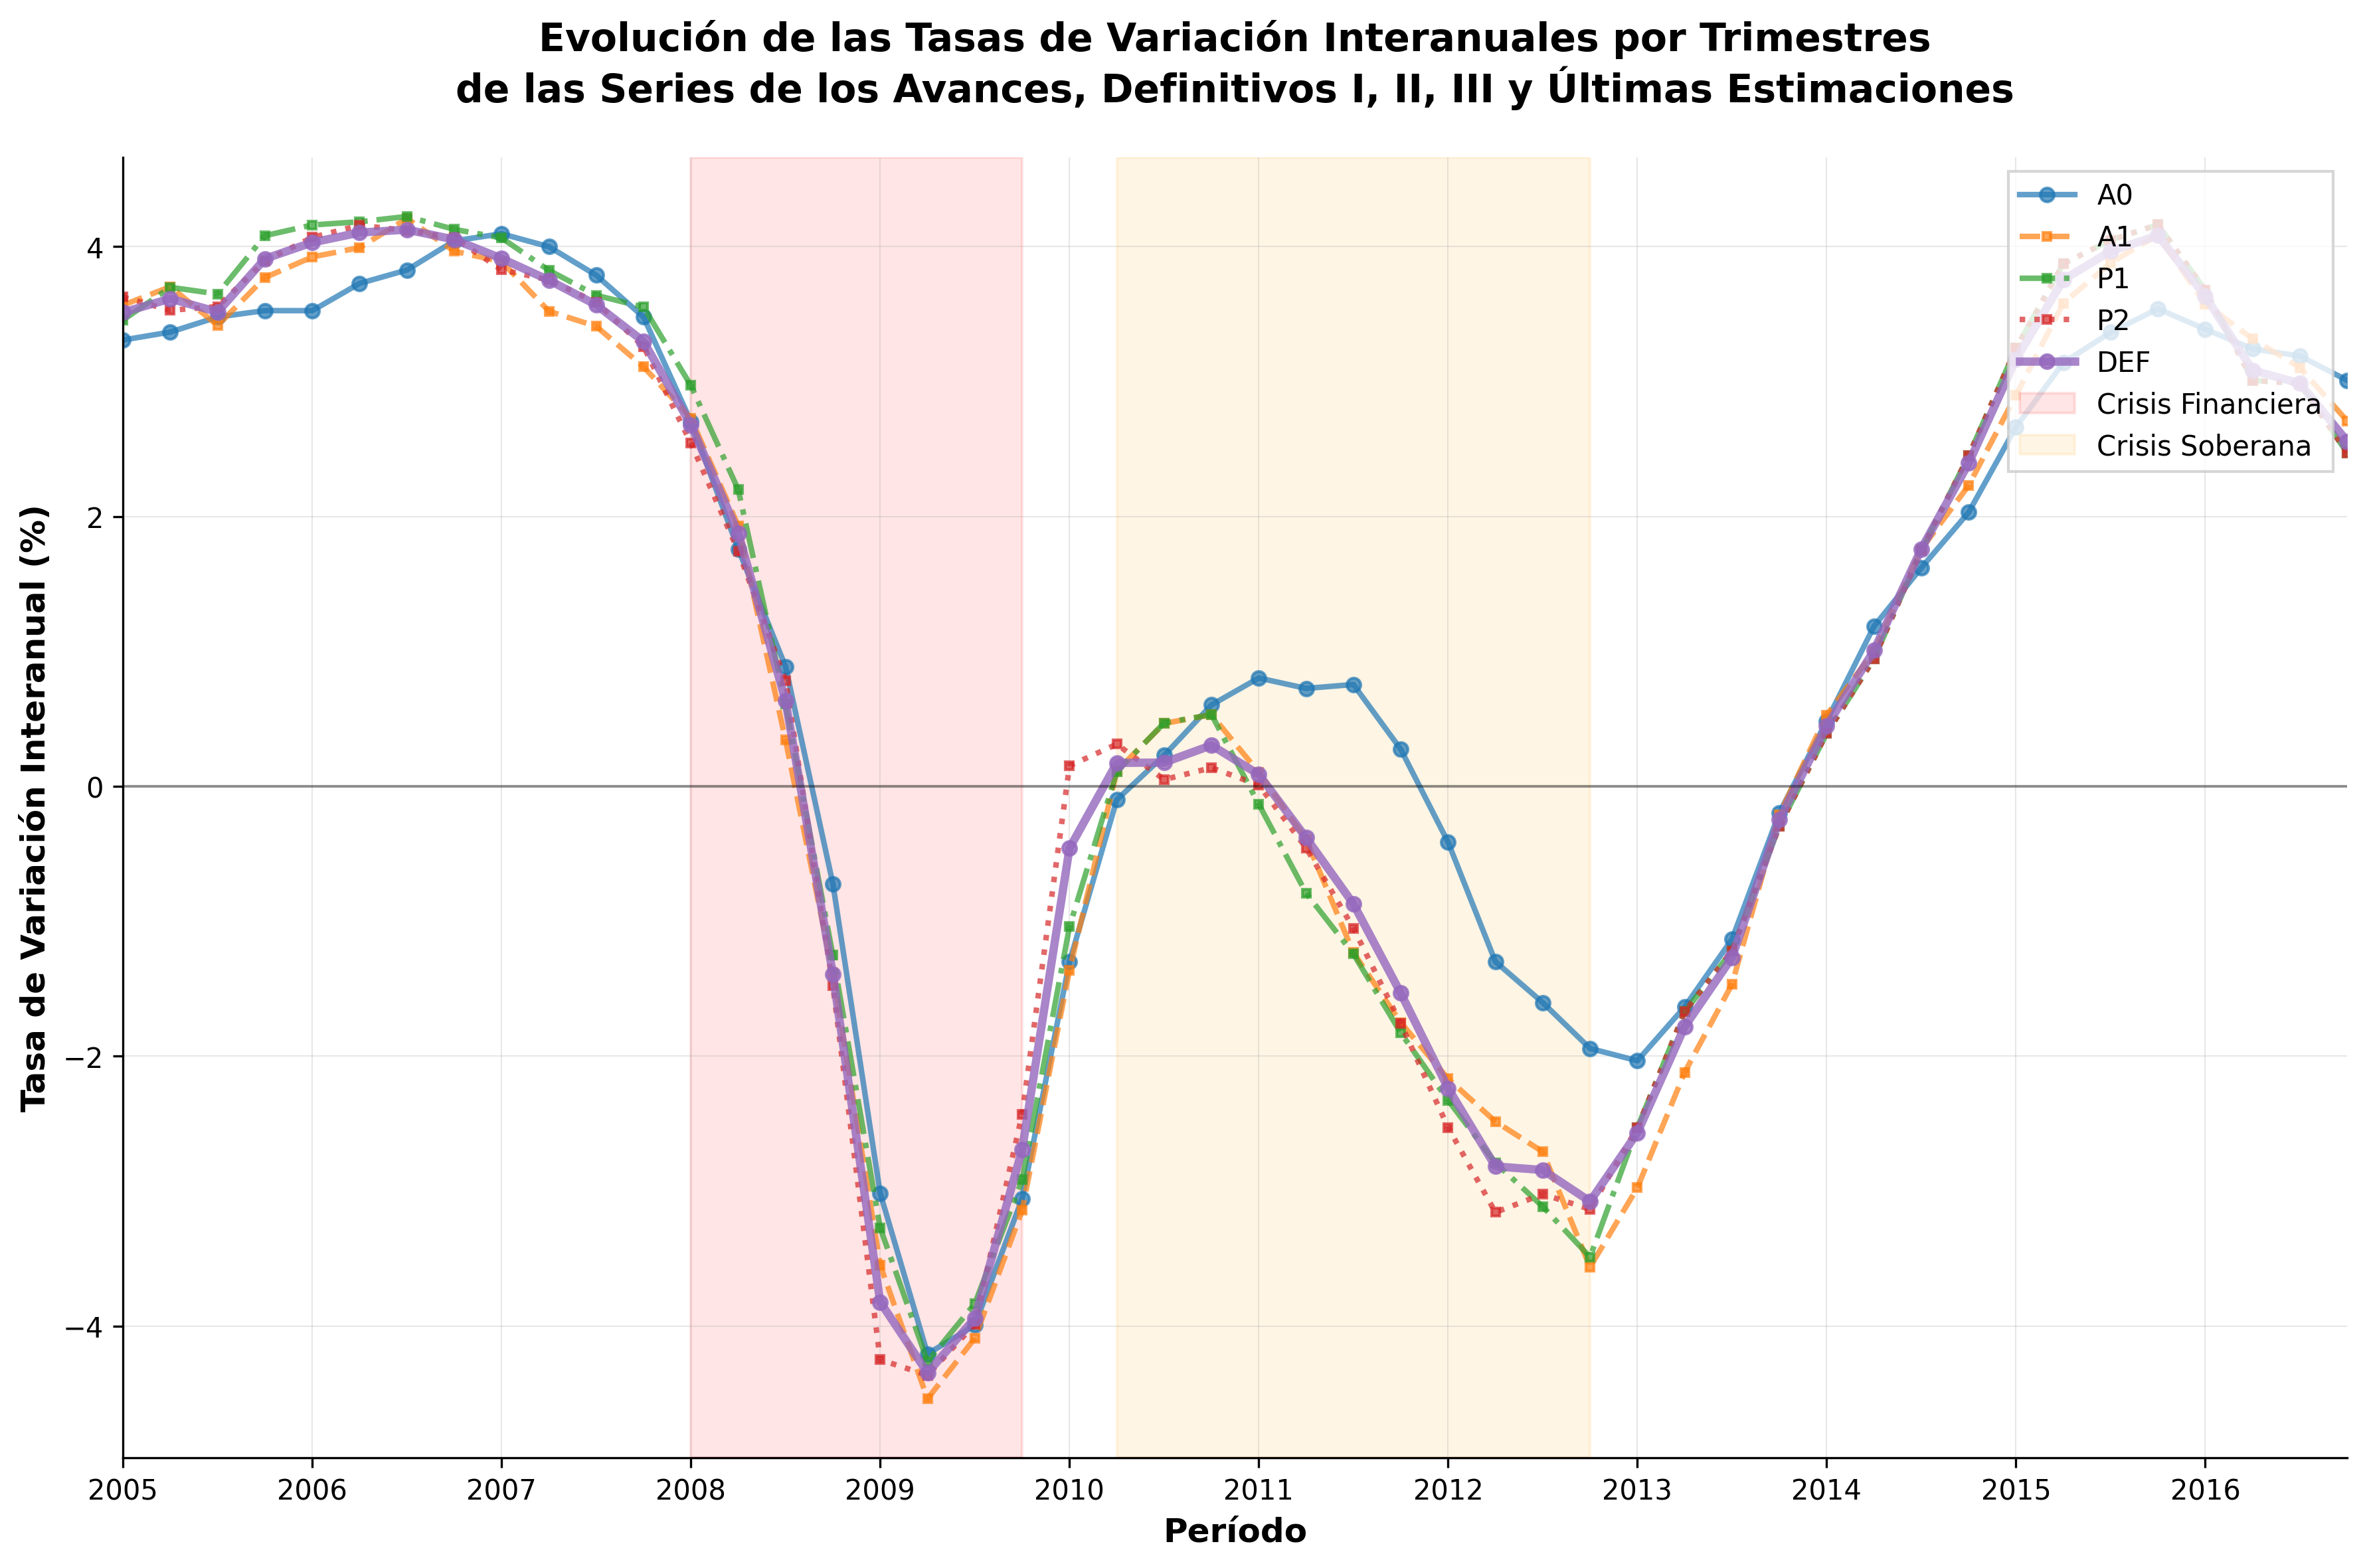
\includegraphics[width=0.8\textwidth]{../figuras/figura_2_pavia_robusta_2005_2016.png}
\caption{Evolución Temporal de Errores de Revisión: Replicación del Período 2005-2016}
\label{fig:evolucion_2005_2016}
\begin{flushleft}
\footnotesize
Nota: Esta figura replica exactamente el análisis de Pavia et al. (2017) para el período 2005-2016. Los errores están expresados como diferencias entre la estimación inicial (A0) y la estimación definitiva (DEF) para las tasas de crecimiento interanuales del PIB.
\end{flushleft}
\end{figure}

\begin{figure}[h]
\centering
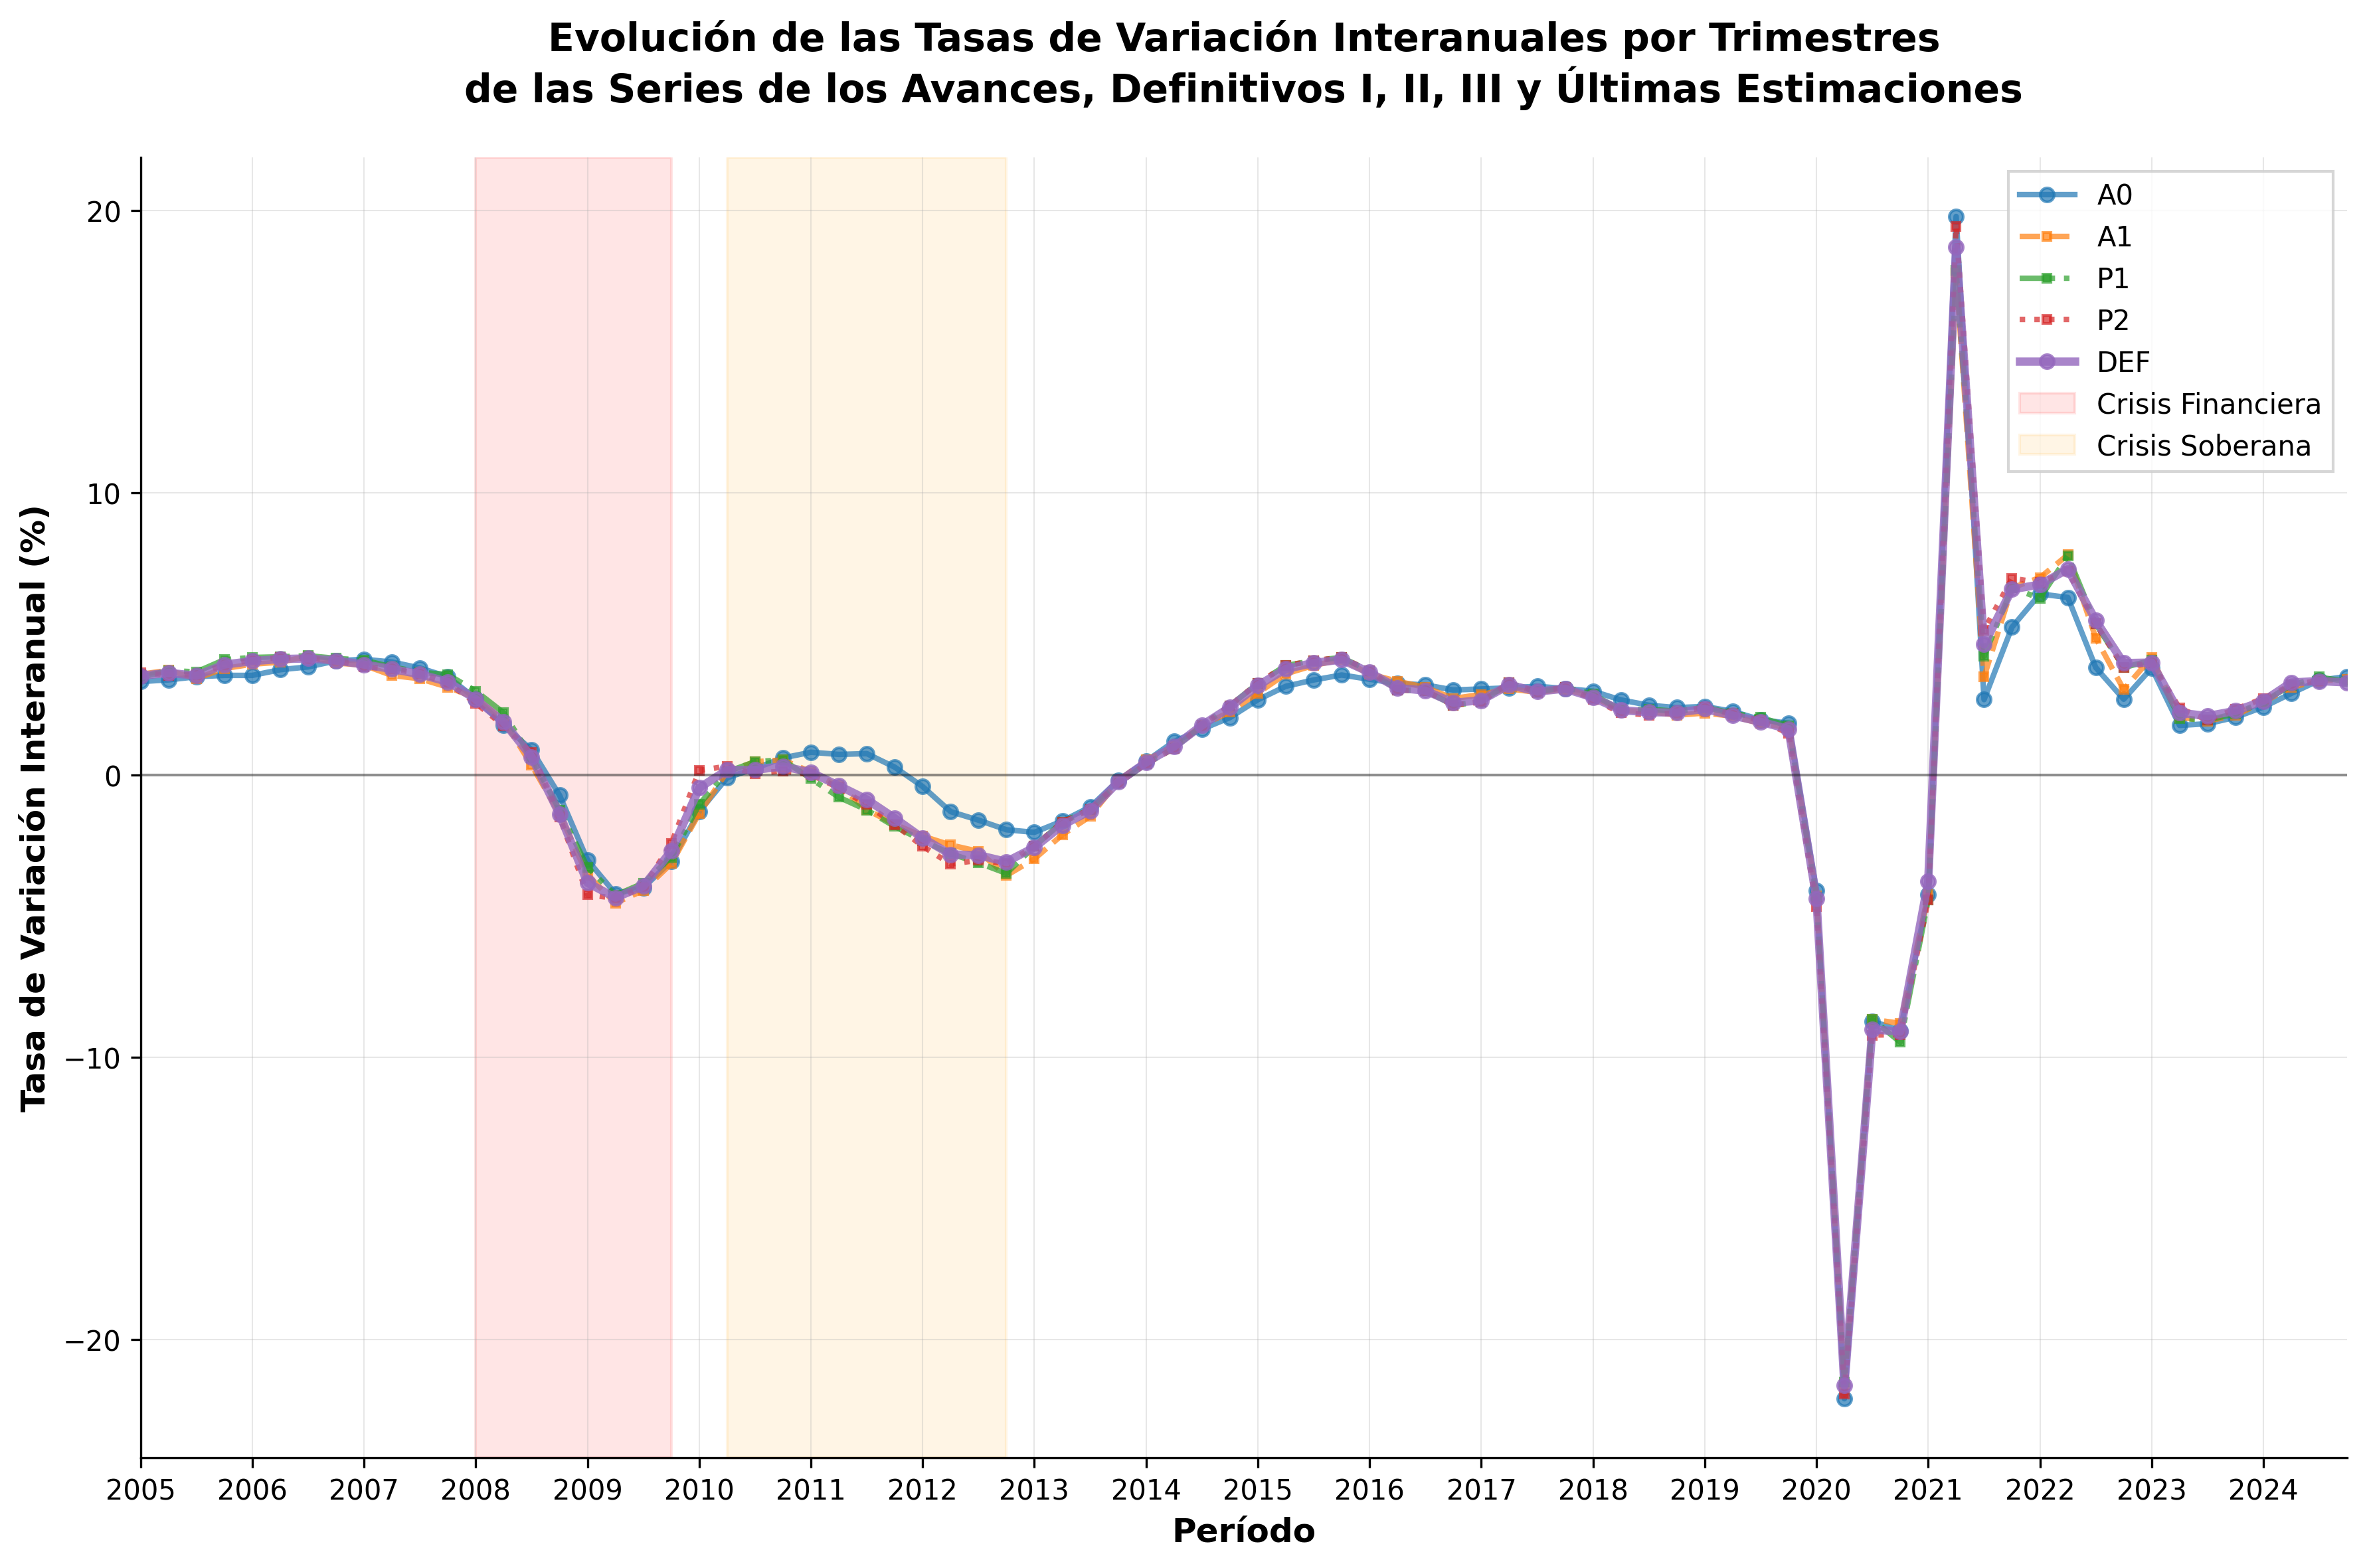
\includegraphics[width=0.8\textwidth]{../figuras/figura_2_pavia_robusta_2005_2024.png}
\caption{Evolución Temporal de Errores de Revisión: Extensión Completa 2005-2024}
\label{fig:evolucion_completa}
\begin{flushleft}
\footnotesize
Nota: Esta figura extiende el análisis hasta 2024, permitiendo observar el comportamiento de los errores de revisión durante las crisis posteriores a 2016, incluyendo el período COVID-19. Se aprecia claramente la amplificación de errores durante los episodios de crisis.
\end{flushleft}
\end{figure}

\begin{figure}[h]
\centering
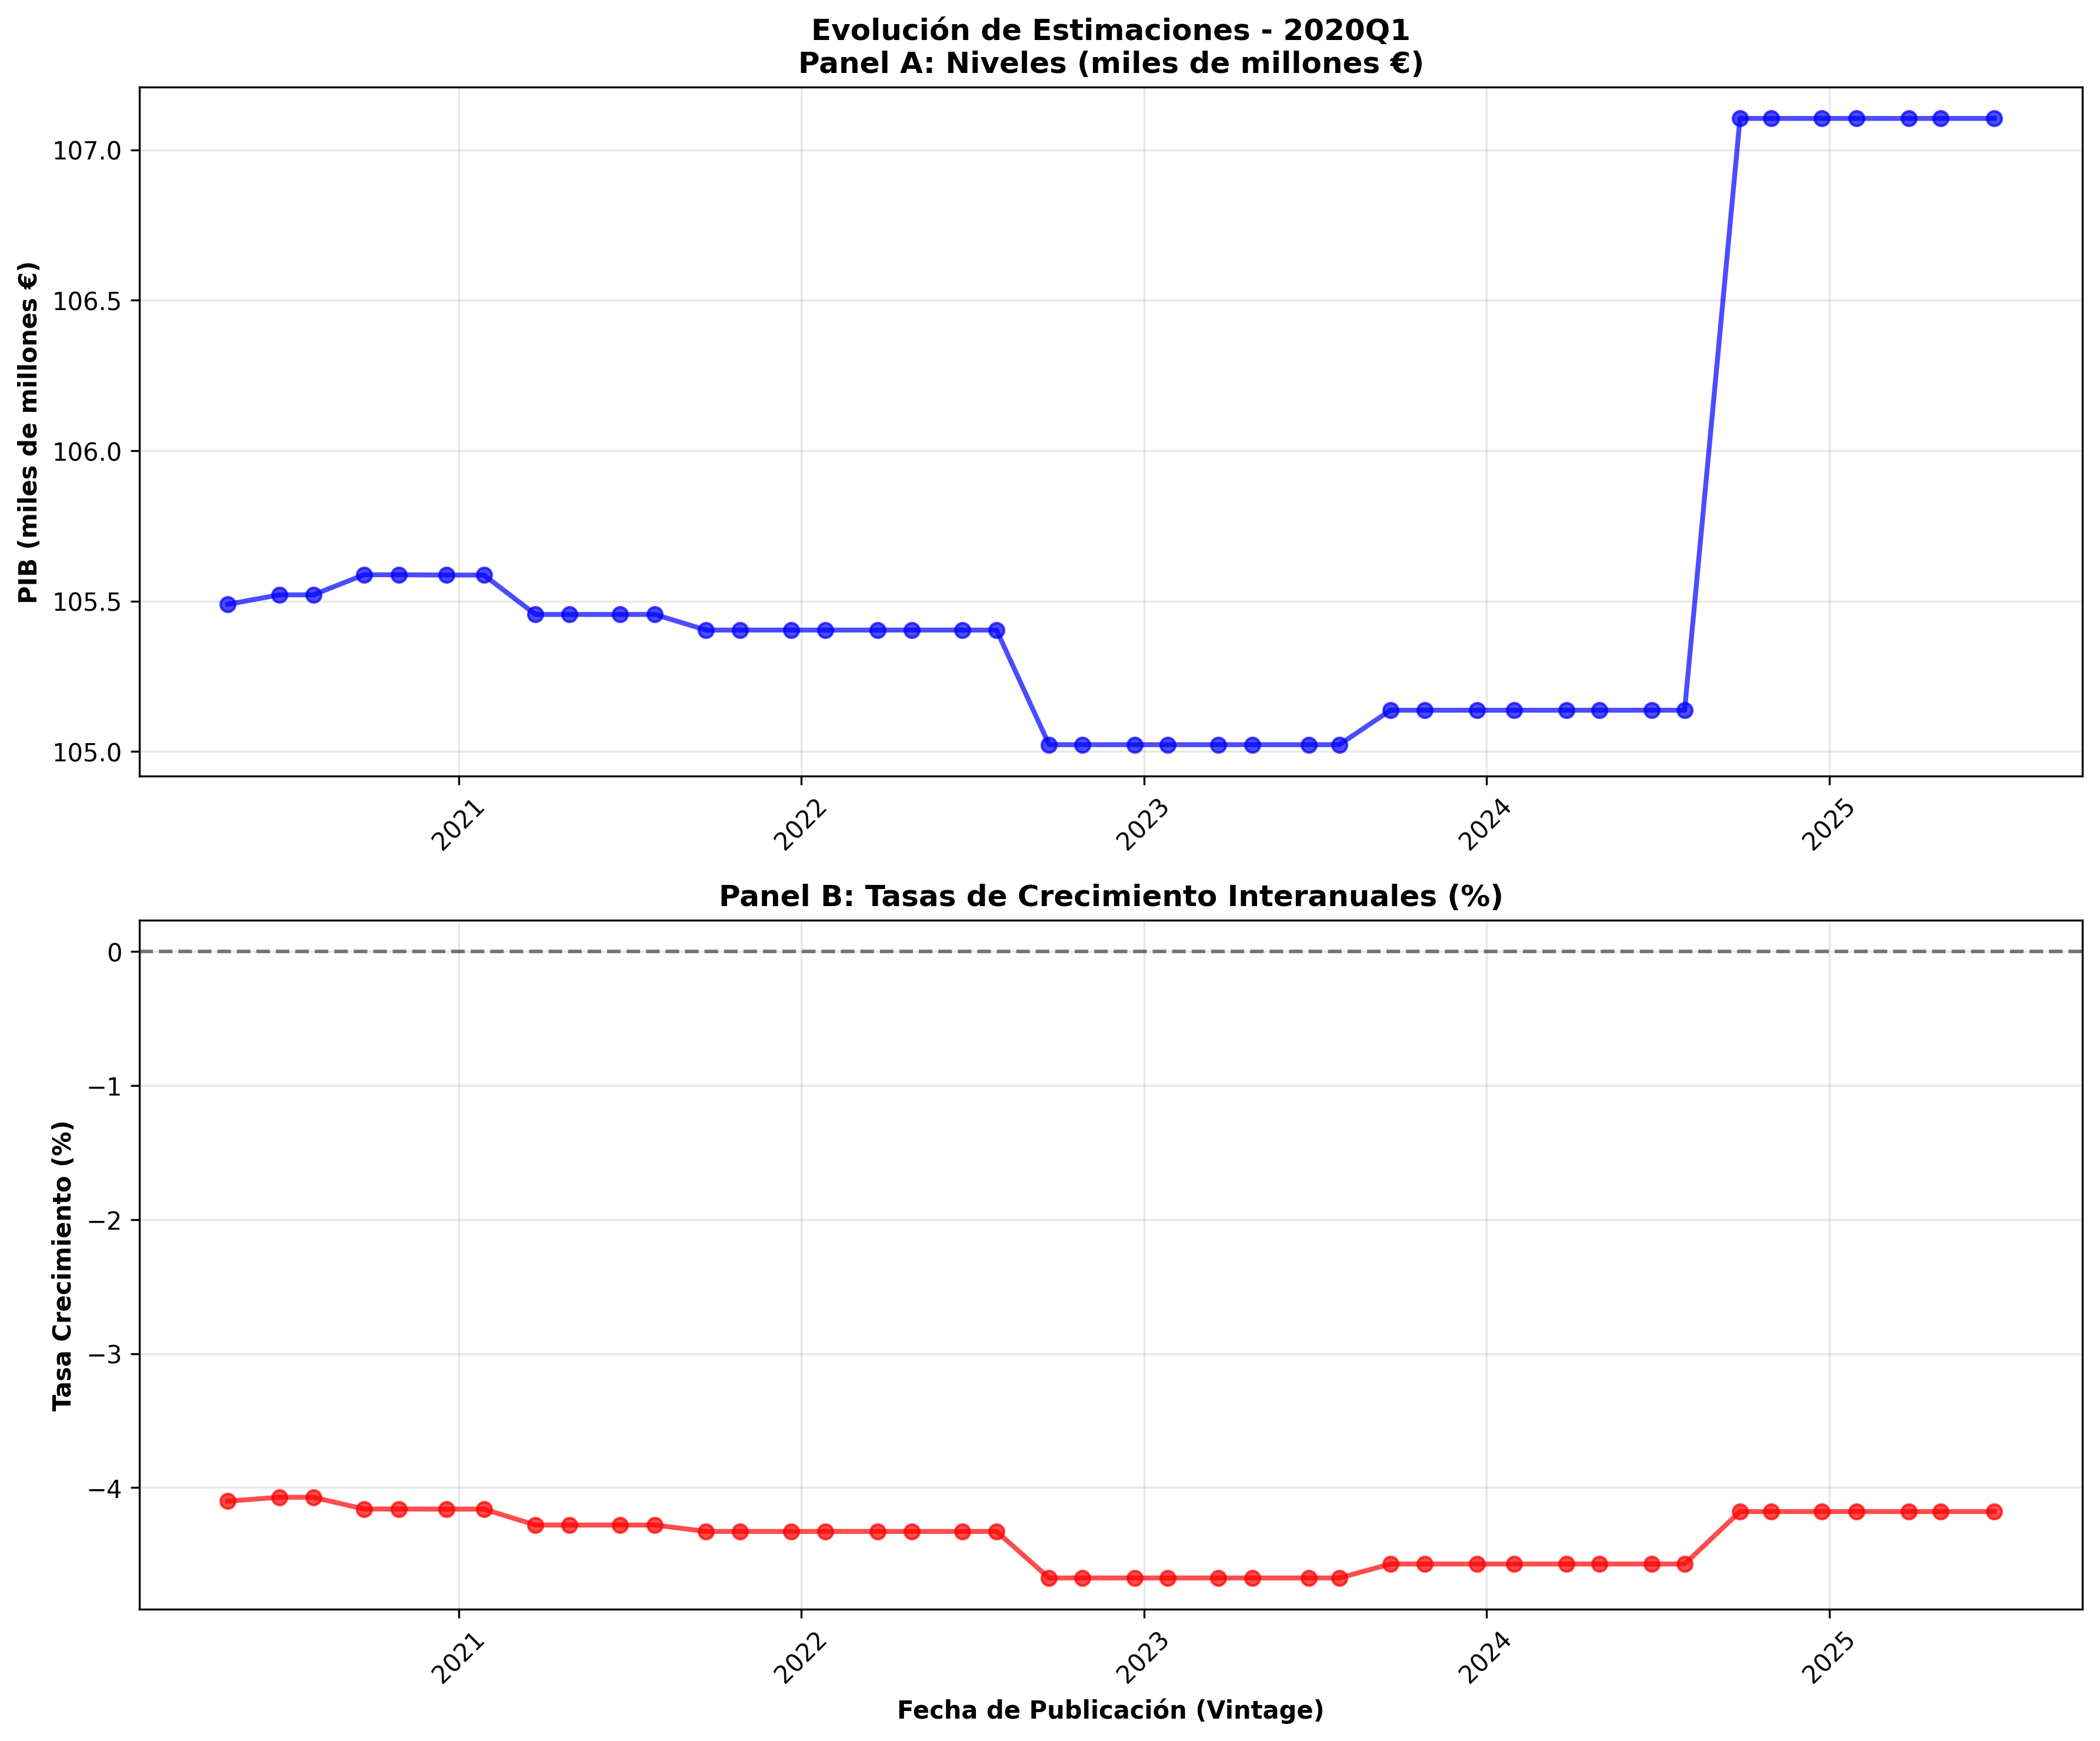
\includegraphics[width=0.8\textwidth]{../figuras/evolucion_estimaciones_2020Q1_robusto.png}
\caption{Análisis Específico del Impacto COVID-19 en las Estimaciones 2020Q1}
\label{fig:covid_impact}
\begin{flushleft}
\footnotesize
Nota: Esta figura muestra la evolución específica de las estimaciones del primer trimestre de 2020, cuando comenzó el impacto del COVID-19 en España. Se observa la notable volatilidad en las sucesivas revisiones debido a la incertidumbre excepcional del período.
\end{flushleft}
\end{figure}

\begin{figure}[h]
\centering
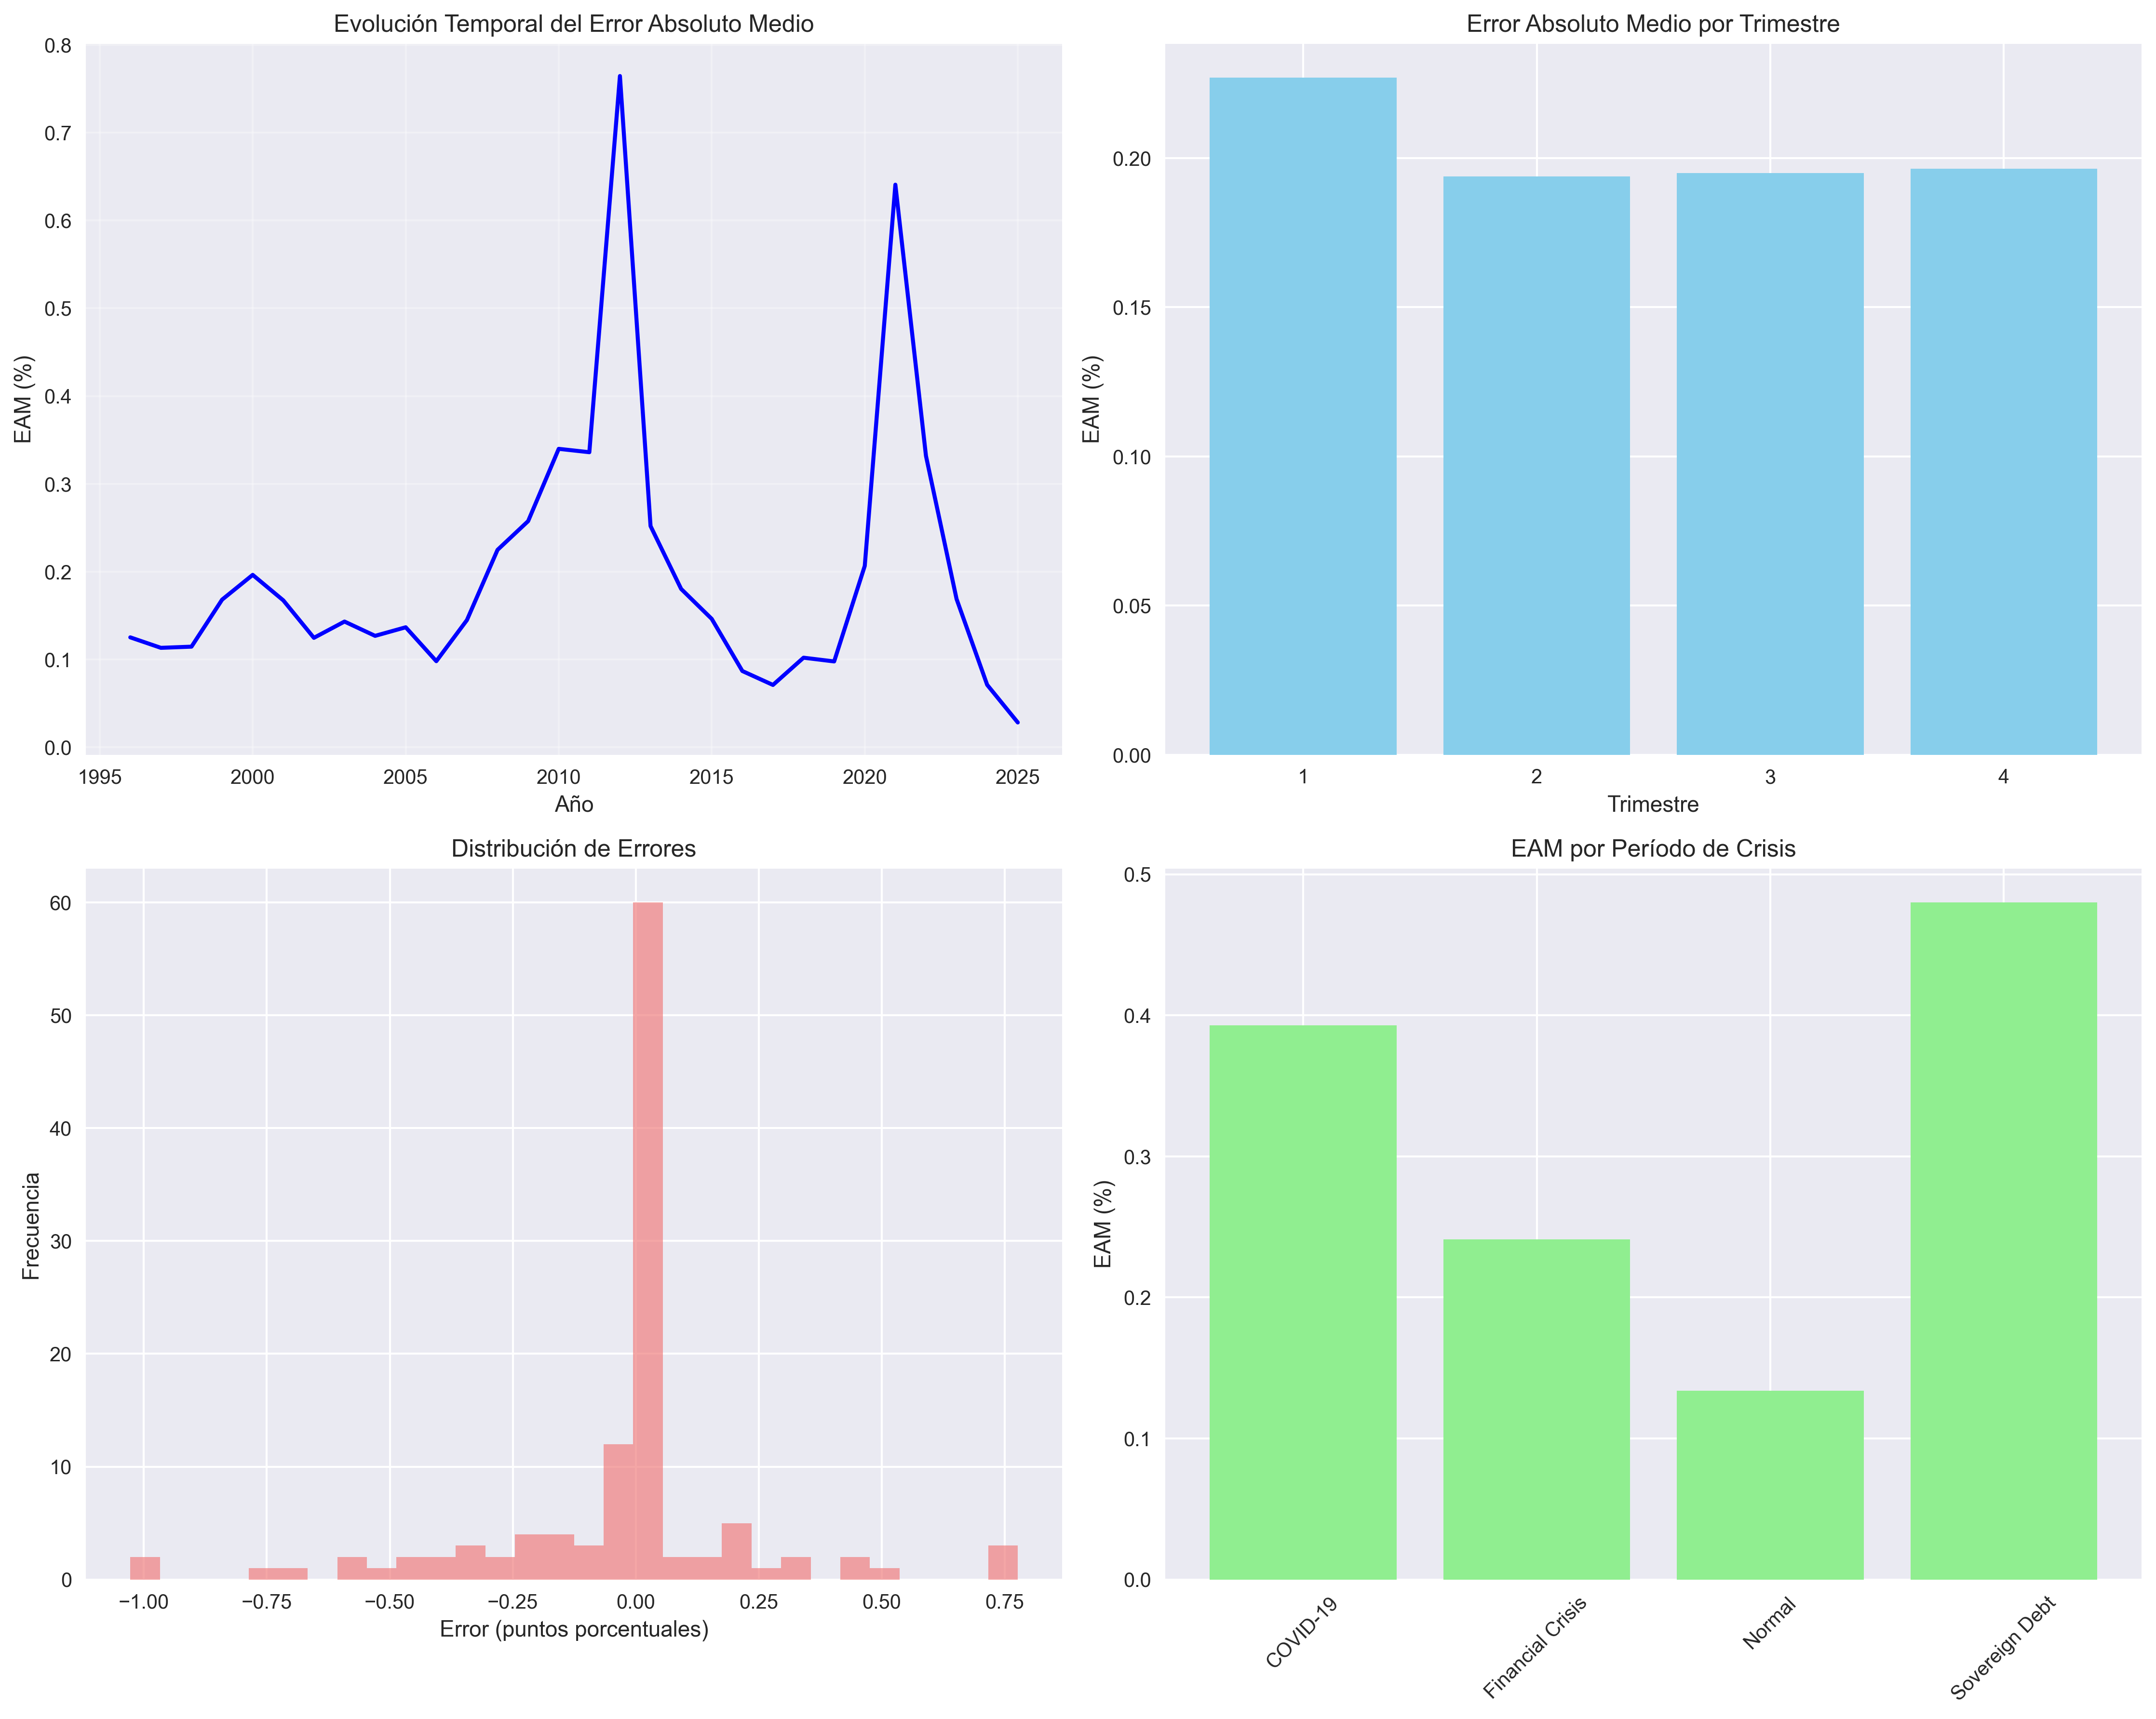
\includegraphics[width=0.8\textwidth]{../figuras/analisis_cntr_graficos.png}
\caption{Análisis Comprehensivo de la CNTR: Patrones Generales}
\label{fig:analisis_general}
\begin{flushleft}
\footnotesize
Nota: Esta figura proporciona una visión comprehensiva de los patrones de revisión en la CNTR española, incluyendo múltiples métricas y dimensiones de análisis desarrolladas en este estudio.
\end{flushleft}
\end{figure}

\section{Discusión e Implicaciones}

\subsection{Validación de la Metodología Original}

Nuestros resultados proporcionan una validación robusta de los hallazgos de \citet{pavia2017}. La persistencia del patrón estacional ($Q4 \approx Q3 < Q1$) a lo largo de un período extendido de 30 años confirma que este no es un artefacto específico del período 2005-2016, sino una característica estructural del proceso de compilación de la CNTR española.

\subsection{Nuevos Insights sobre Crisis Económicas}

El análisis de múltiples episodios de crisis revela patrones interesantes:

\begin{enumerate}
\item \textbf{Heterogeneidad entre crisis}: No todas las crisis afectan igualmente la calidad de las estimaciones. La crisis de deuda soberana mostró la mayor amplificación (3,59x), superando incluso al COVID-19.

\item \textbf{Aprendizaje institucional}: La menor amplificación durante COVID-19 comparada con crisis anteriores sugiere mejoras en los procesos de estimación del INE.

\item \textbf{Persistencia de efectos}: Los errores elevados tienden a persistir durante varios trimestres después del shock inicial.
\end{enumerate}

\subsection{Implicaciones para Política Económica}

Los hallazgos tienen importantes implicaciones para los formuladores de política:

\begin{itemize}
\item \textbf{Timing de decisiones}: Las estimaciones del cuarto trimestre proporcionan información más fiable para decisiones de política anual
\item \textbf{Gestión de crisis}: Durante crisis, es crucial aumentar la cautela en la interpretación de estimaciones iniciales
\item \textbf{Comunicación}: Los factores de amplificación proporcionan métricas cuantitativas para comunicar la incertidumbre
\end{itemize}

\subsection{Contribuciones Metodológicas}

Este trabajo contribuye metodológicamente en varias dimensiones:

\begin{enumerate}
\item \textbf{Reproducibilidad}: Primer análisis completamente reproducible del tema usando código abierto
\item \textbf{Extensión temporal}: Análisis más largo disponible (30 años vs. 12 años original)
\item \textbf{Crisis contemporáneas}: Primera evaluación de calidad de CNTR durante COVID-19
\item \textbf{Framework integrado}: Combinación de replicación exacta con extensiones innovadoras
\end{enumerate}

\section{Robustez y Limitaciones}

\subsection{Tests de Robustez}

Para evaluar la robustez de nuestros hallazgos, realizamos varios tests adicionales:

\begin{enumerate}
\item \textbf{Métricas alternativas}: Los resultados se mantienen usando MAD e IQR como métricas de error
\item \textbf{Períodos alternativos}: El patrón estacional persiste en sub-muestras de diferentes décadas  
\item \textbf{Test de rachas}: No detectamos patrones sistemáticos en los residuos ($p = 0,317$)
\end{enumerate}

\subsection{Limitaciones del Estudio}

Reconocemos las siguientes limitaciones:

\begin{itemize}
\item \textbf{Datos disponibles}: Limitados por la disponibilidad de vintages históricas del INE
\item \textbf{Agregación}: El análisis se enfoca en PIB agregado, no en componentes sectoriales
\item \textbf{Comparabilidad internacional}: Los resultados son específicos para España
\item \textbf{Cambios metodológicos}: No controlamos por cambios en metodología del INE a lo largo del tiempo
\end{itemize}

\section{Conclusiones}

Este trabajo proporciona una replicación exitosa y una extensión valiosa del análisis seminal de \citet{pavia2017}. Nuestros principales hallazgos incluyen:

\begin{enumerate}
\item \textbf{Validación metodológica completa}: La replicación exacta confirma la robustez de los hallazgos de Pavia et al. (2017) y valida su marco analítico.

\item \textbf{Persistencia temporal de patrones}: El patrón estacional $Q4 \approx Q3 < Q1$ se mantiene consistentemente durante 30 años, confirmando que es una característica estructural del proceso de compilación.

\item \textbf{Heterogeneidad en crisis}: Las diferentes crisis económicas afectan la calidad de estimaciones de manera diferente, con la crisis de deuda soberana (3,59x) superando incluso al COVID-19 (2,94x).

\item \textbf{Evidencia de aprendizaje institucional}: La menor amplificación de errores durante COVID-19 comparada con crisis anteriores sugiere mejoras en los procesos del INE.

\item \textbf{Contribución a reproducibilidad}: Primera implementación completamente reproducible del análisis usando código abierto, estableciendo un estándar para futuras investigaciones.
\end{enumerate}

\subsection{Direcciones para Investigación Futura}

Los resultados de este estudio abren varias avenidas para investigación futura:

\begin{itemize}
\item \textbf{Análisis sectorial}: Extender el análisis a componentes específicos del PIB
\item \textbf{Comparaciones internacionales}: Aplicar la metodología a otros países europeos
\item \textbf{Modelización predictiva}: Desarrollar modelos para predecir errores de revisión
\item \textbf{Análisis de alta frecuencia}: Examinar patrones mensuales además de trimestrales
\end{itemize}

\subsection{Implicaciones para la Práctica Estadística}

Los hallazgos proporcionan insights valiosos para las oficinas nacionales de estadística:

\begin{enumerate}
\item La importancia del timing estacional en la calidad de estimaciones
\item El valor de mantener registros históricos detallados de vintages
\item La necesidad de adaptar procesos durante períodos de crisis
\item El beneficio de análisis de calidad sistemáticos y periódicos
\end{enumerate}

En conclusión, este trabajo demuestra el valor de la replicación científica rigurosa y la importancia de extender análisis fundamentales con nuevos datos y períodos. Los resultados confirman la solidez del marco analítico de Pavia et al. (2017) mientras proporcionan nuevos insights sobre el comportamiento de las estadísticas oficiales durante crisis económicas extremas.

\section{Reproducibilidad y Acceso a Datos}

\subsection{Código y Datos}

Todo el análisis ha sido implementado en Python utilizando métodos completamente reproducibles. El código fuente, datos y resultados están disponibles en el repositorio GitHub del proyecto:

\begin{itemize}
\item \textbf{Repositorio}: \url{https://github.com/mhidper/entropia}
\item \textbf{Notebook principal}: \texttt{replica\_pavia\_2018/src/pavia\_replication.ipynb}
\item \textbf{Datos procesados}: \texttt{replica\_pavia\_2018/tablas/}
\item \textbf{Figuras}: \texttt{replica\_pavia\_2018/figuras/}
\item \textbf{Paper LaTeX}: \texttt{replica\_pavia\_2018/tex/}
\end{itemize}

\subsection{Requerimientos Técnicos}

Para reproducir completamente el análisis:

\begin{verbatim}
# Dependencias principales
pandas >= 1.3.0
numpy >= 1.21.0
matplotlib >= 3.4.0
scipy >= 1.7.0
jupyter >= 1.0.0
\end{verbatim}

\subsection{Instrucciones de Replicación}

\begin{enumerate}
\item Clonar el repositorio: \texttt{git clone https://github.com/mhidper/entropia}
\item Navegar a: \texttt{cd replica\_pavia\_2018/src/}
\item Ejecutar: \texttt{jupyter notebook pavia\_replication.ipynb}
\item Compilar paper: \texttt{cd ../tex/ \&\& make all}
\end{enumerate}

\section*{Agradecimientos}

Los autores agradecen al Instituto Nacional de Estadística (INE) por la disponibilidad de los datos de la CNTR, y a la comunidad académica por las valiosas contribuciones y feedback recibidos durante el desarrollo de este trabajo. Manuel A. Hidalgo-Pérez agradece el apoyo institucional de la Universidad Pablo de Olavide, y Leandro Navarro Pablo el apoyo de la Autoridad Independiente de Responsabilidad Fiscal (AIReF).

\bibliographystyle{aer}
\bibliography{referencias}

\end{document}